% !Mode:: "TeX:UTF-8"
\title{公交安全管理系统报告}
\author{江昱峰 21009200038} 
\documentclass {article}
\usepackage[UTF8]{ctex}
\usepackage{graphicx}
\usepackage{float}
\usepackage{hyperref}
\usepackage{makecell}
\usepackage{listings}
\begin{document}
	%\begin{sloppypar}
	\maketitle{}
	\section{需求分析(系统数据和功能)}
		\subsection{后台数据库}
			设计公交安全管理系统,推荐使用openGauss。    
			
			数据库的有关语义如下:
			\begin{enumerate}
				\item 公交公司有若干个车队,每个车队下有若干条线路;
				\item 公交公司有若干辆汽车,每辆车属于一条线路;
				\item 每个车队有一名队长,他只有管理工作,不开车;
				\item 每条线路有若干名司机,其中有一名路队长,除开车外,还承担管理工作;
				\item 每名司机只在一条线路上开车;
				\item 司机开车时会产生违章,包含:闯红灯、未礼让斑马线、压线、违章停车等;
				\item 队长、路队长负责将司机的违章信息输入到系统,包含:司机、车辆、车队、线路、站点、时间、违章等。
			\end{enumerate}
			
		\subsection{前台程序}
			开发一个公交安全管理系统来对数据库进行访问,可以使用Java、Python、C等集成开发环境。    
			
			系统实现功能如下:
			\begin{enumerate}
				\item 录入司机基本信息,如工号、姓名、性别等;
				\item 录入汽车基本信息,如车牌号、座数等;
				\item 录入司机的违章信息;
				\item 查询某个车队下的司机基本信息;
				\item 查询某名司机在某个时间段的违章详细信息;
				\item 查询某个车队在某个时间段的违章统计信息,如:2次闯红灯、4次未礼让斑马线等。
			\end{enumerate}
			
			除此之外,我还根据队长、路队长、司机的身份差异,针对不同的功能分别设置了\textbf{三级权限}。
			
		\subsection{注意事项}
			\begin{enumerate}
				\item 在数据库的设计过程中需要运用规范化理论,避免出现插入异常、删除异常、数据冗余等问题;
				\item 必须设定关系的完整性规则,如实体完整性(例如设置主码),参照完整性(例如设置外码和对应的主码),用户自定义完整性(例如性别只能为“男”或“女”);
				\item 使用索引来加快查询的速度;
				\item 使用视图、函数、存储过程来简化系统的设计;
				\item 使用数据库设计工具,例如:ERWin,PowerDesigner实习重点在于后台数据库的设计,对于前台程序的开发,能够实现系统功能即可,不要把大量时间花费在界面设计和不必要的代码上。
			\end{enumerate}
		
	\section{概念结构设计(E-R图设计)}
		首先,我根据后台数据库要求的数据库语义关系和前台程序要求的数据属性分析、设计出概念结构,并用ERwin软件设计了如下所示的E-R图:
		\begin{figure}[H]
			\centering
			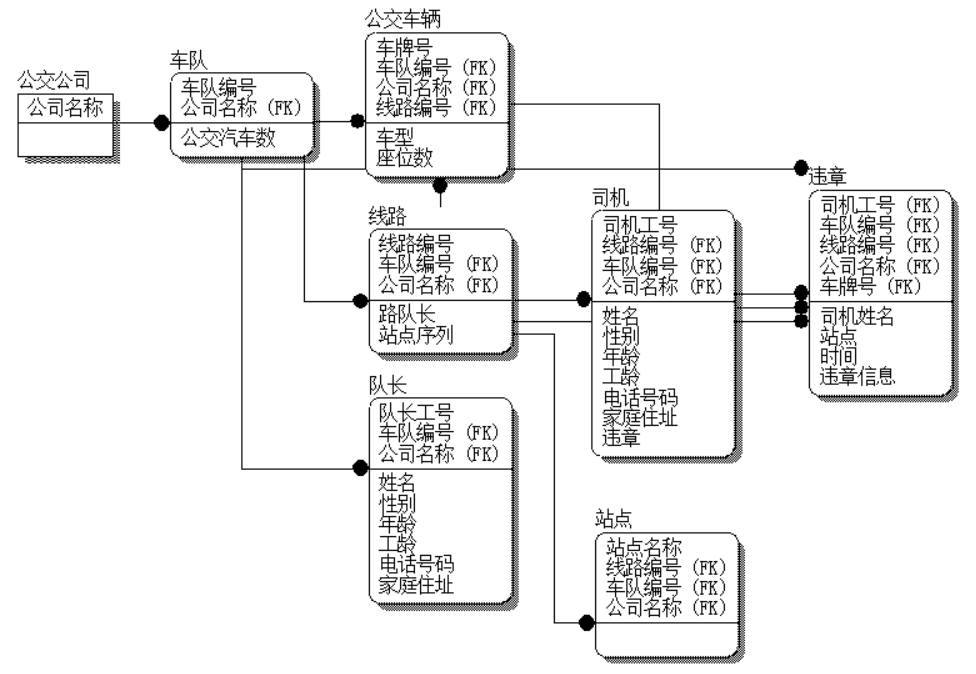
\includegraphics[width=4.5in]{figures/fig1.png}
			\caption{概念结构E-R图}
		\end{figure}
	
		图中,除了后台数据库要求的数据库语义关系之外,还包括车队和公交汽车的一对多关系、线路和站点的关系等。每个实体的属性均已列出,在前台程序要求录入的基本信息的基础上,我还加入了许多属性,使得实体信息更为完整。事实上,除了E-R图中展示出的关系,还有许多隐藏关系,但由于存在意义较低,图中便没有展示。
	
	\section{逻辑结构设计(E-R图转换为关系模型)}
		基于上一部分的概念结构E-R图,我将转换为关系模型,从而设计了对应的逻辑结构如下,其中加粗的属性为主码:
		\begin{itemize}
			\item 车队组成关系:车队组成(\textbf{车牌号},车队编号);
			\item 车队驾驶线路关系:车队驾驶线路(\textbf{车队编号},线路编号,站点序列);
			\item 车辆驾驶线路关系:车辆驾驶线路(\textbf{车牌号},线路编号);
			\item 队长对于车队的管理关系:队长管理车队(\textbf{队长工号},车队编号);
			\item 队长对于司机的管理关系:队长管理司机(\textbf{司机工号},队长工号);
			\item 路队长对于线路的管理关系:路队长管理车队(\textbf{路队长工号},线路编号);
			\item 路队长对于司机的管理关系:路队长管理司机(\textbf{司机工号},路队长工号);
			\item 公交汽车驾驶线路关系:驾驶线路(\textbf{车牌号},线路编号,座位数,站点序列);
			\item 司机驾驶线路关系:司机驾驶线路(\textbf{司机工号},线路编号);
			\item 线路途经站点关系:线路途经站点(\textbf{线路编号},站点序列元组)。
		\end{itemize}
		其中,对于一对多(1对n)关系的转换,主要有两种方法,第一种方法是对应的关系模式中,其主码不再是任一实体的主码就可以,而是必须指定n端的主码为关系模式的主码;第二种方法是将1端的主码加到n端的关系模式中,而且n端的主码仍然为该关系模式中的主码。此处我用的是使用更为广泛的后者。
	
	\section{程序开发环境及应用环境}
		关于程序开发环境及应用环境,后台数据库对应的是MySQL 8.0、JetBrains的DataGrip 2023.2,前台管理程序对应的是VSCode。二者对应的编程语言分别为SQL和Python 3.10。具体代码见附录部分。
	
	\section{应用程序设计中遇到的问题及解决方法}
		应用程序设计中,我遇到了许多问题,除了一般的程序语法问题之外,还有一些比较典型、有价值、值得反思的问题,具体问题及对应的解决方法如下:
		
		后台数据库设计部分:
		\begin{itemize}
			\item 具体问题:为了设定参照完整性,我对每个数据表都设置了外码和对应的主码,这使得多个数据表在创建时存在相应的先后顺序要求,不能完全按照自己想要的顺序创建;解决方法:我借鉴了数据结构与算法中学习到的图论里的拓扑排序算法的思想,通过数据表之间的依赖关系确定了创建的顺序;
			\item 具体问题:我在设计时需要多次运行SQL程序,这使得我在之前运行过程中已经创建好的数据表在之后又重复创建,导致数据冗余报错;解决方法:由于前后创建的数据表内容可能有所不同,相比“先判断要创建的表格是否存在,若存在则不再重复创建”的方法,我采用的是在创建数据表之前先判断该表是否已经存在,若存在则删除,然后再创建的方法,这样既完全解决了数据冗余的问题,又保证了创建的数据表内容是最新的。
		\end{itemize}
	
		前台程序设计部分:
		\begin{itemize}
			\item 具体问题:我在录入信息时,程序和其连接的后台数据库都没有报错,但此插入操作在后台数据库中对应的数据表并没有产生新数据、造成影响;解决方法:在游标cursor执行完SQL命令后,还需要通过commit方法提交事务才能完全生效;
			\item 具体问题:在录入信息时,由于我在后台数据库中设置了外码和对应的主码,此参照完整性对我录入的数据有相应的要求,不能随意地插入数据;解决方法:我先在后台数据库中插入一些数据,然后再基于这些数据,在前台程序中录入信息;
			\item 具体问题:我在通过点击显示框右上角“×”的图标关闭界面、退出系统、终止程序运行时,下一个显示框依旧弹出;解决方法:我额外设计了一个触发器,在点击图标时触发已经预先设定好的变量的变化,进而关闭界面并结束程序运行;
			\item 具体问题:显示查询结果的同时直接弹出了选择继续或退出的界面;解决方法:与上一个问题的解决方法类似,通过设置触发器的方式解决。
		\end{itemize}
	
	\section{总结}
		完成本次上机作业后,我做了以下几点总结:
		\begin{itemize}
			\item 在设计后台数据库之前,需要先设计概念结构(E-R图),并将其转换为关系模型的逻辑结构,从而对数据库各数据表及其属性的相互关系有更全面、严谨的把握;
			\item 设计后台数据库时,需要运用规范化理论,避免出现插入异常、删除异常、数据荣誉等问题。具体的,在创建数据表之前,需要先判断该数据表是否已经存在,防止发生数据冗余问题;
			\item 必须设定关系的完整性规则,如实体完整性(例如设置主码),参照完整性(例如设置外码和对应的主码),用户自定义完整性(例如性别只能为“男”或“女”)。具体的,在创建数据表之前,需要先确定好各数据表的创建顺序,防止发生由外码和对应主码导致的参照完整性问题;
			\item 可以使用索引来加快查询的速度,使用视图、函数、存储过程来简化系统的设计;
			\item 设计前台程序时,在录入信息时,不能随意地插入数据,需要符合相应的完整性规则;
			\item 在录入信息之后,需要通过commit方法提交事务才能使得插入语句完全生效。
		\end{itemize}
	
	\section{附录:建立数据库和应用程序的主要代码}
		\subsection{建立数据库的主要代码}
			\begin{lstlisting}[language=SQL]
-- 创建数据库
-- 创建数据库
DROP DATABASE IF EXISTS bus; -- 若数据库已存在则删除
CREATE DATABASE bus;
USE bus;

-- 删除现有数据库
DROP TABLE IF EXISTS Route;
DROP TABLE IF EXISTS Driver;
DROP TABLE IF EXISTS Convoy;
DROP TABLE IF EXISTS Leader;
DROP TABLE IF EXISTS Bus;
DROP TABLE IF EXISTS Illegal;

-- 创建数据表(包括实体完整性、参照完整性、用户自定义完整性等完整性规则)
CREATE TABLE Leader -- 队长表
    (number_job INT PRIMARY KEY NOT NULL,
     name CHAR(8) NOT NULL,
     sex CHAR(2) NOT NULL CHECK (sex IN ('男','女')),
     age INT NOT NULL,
     phone_number BIGINT NOT NULL CHECK (phone_number BETWEEN 10000000000 AND 99999999999) UNIQUE,
     address CHAR(50) NOT NULL);

CREATE TABLE Convoy -- 车队表
    (number_convoy INT PRIMARY KEY NOT NULL, -- 车队编号
     number_job_leader INT NOT NULL,
     FOREIGN KEY (number_job_leader) REFERENCES Leader(number_job)); -- 队长工号

CREATE TABLE Route -- 线路表
    (number_route INT PRIMARY KEY NOT NULL, -- 线路编号
     number_job_routeleader INT NOT NULL); -- 路队长工号

CREATE TABLE Driver -- 司机表(包括路队长,但不包括队长)
    (number_job INT PRIMARY KEY NOT NULL, -- 工号
     number_route INT NOT NULL, -- 线路编号
     name CHAR(8) NOT NULL,
     sex CHAR(2) NOT NULL CHECK (sex IN ('男','女')),
     age INT NOT NULL CHECK (age BETWEEN 18 AND 60),
     phone_number BIGINT NOT NULL UNIQUE CHECK(phone_number BETWEEN 10000000000 AND 99999999999),
     address CHAR(50) NOT NULL,
     FOREIGN KEY (number_route) REFERENCES Route(number_route));

CREATE TABLE Bus -- 公交汽车表
    (number_bus CHAR(10) PRIMARY KEY NOT NULL, -- 车牌号
     number_convoy INT NOT NULL, -- 车队编号
     number_route INT NOT NULL, -- 线路编号
     size INT NOT NULL, -- 座数
     type CHAR(20) NOT NULL, -- 车型
     FOREIGN KEY (number_convoy) REFERENCES Convoy (number_convoy),
     FOREIGN KEY (number_route) REFERENCES Route (number_route));

CREATE TABLE Illegal -- 违章信息表
    (number_job INT NOT NULL, -- 工号
     name CHAR(30) NOT NULL, -- 姓名
     number_bus CHAR(10) NOT NULL, -- 车牌号
     number_convoy INT NOT NULL, -- 车队编号
     number_route INT NOT NULL, -- 线路编号
     site CHAR(20) NOT NULL, -- 站点
     time DATETIME NOT NULL, -- 时间
     illegal CHAR(20) NOT NULL, -- 违章信息
     FOREIGN KEY (number_job) REFERENCES Driver (number_job),
     FOREIGN KEY (number_bus) REFERENCES Bus (number_bus),
     FOREIGN KEY (number_convoy) REFERENCES Convoy (number_convoy),
     FOREIGN KEY (number_route) REFERENCES Route (number_route)); -- 违章表

-- 创建索引来加快查询的速度
CREATE INDEX index_convoy ON Convoy (number_convoy ASC) ;
CREATE INDEX index_route ON Route (number_route ASC);
CREATE INDEX index_leader ON Leader (number_job ASC);
CREATE INDEX index_bus ON Bus (number_bus ASC);
CREATE INDEX index_driver ON Driver (number_job ASC);

-- 创建视图来简化系统的设计
CREATE VIEW Route_leader
	AS
	SELECT * 
	FROM Driver
	WHERE number_job IN
	(SELECT number_job_routeleader FROM Route);

-- 录入信息
INSERT INTO Leader VALUES (1,'江昱峰','男',19,13914250795,'陕西省西安市西安电子科技大学南校区海棠十号楼二区302左室');
INSERT INTO Leader VALUES (2,'轻井泽','女',22,13921190025,'陕西省西安市西安电子科技大学南校区丁香十四号楼一区606右室');
INSERT INTO Convoy VALUES (1,1);
INSERT INTO Convoy VALUES (2,2);
INSERT INTO Route VALUES (1,3);
INSERT INTO Route VALUES (2,4);
INSERT INTO Bus VALUES ('陕A B107R',1,1,16,'新能源公交车');
INSERT INTO Bus VALUES ('陕A 12345',2,2,20,'混合动力公交车');
INSERT INTO Driver VALUES (3,1,'汪文轩','男',20,13914112452,'陕西省西安市西安电子科技大学南校区海棠十号楼二区302左室');
INSERT INTO Driver VALUES (4,2,'王俞钦','男',21,13914112453,'陕西省西安市西安电子科技大学南校区海棠十号楼二区304右室');
INSERT INTO Driver VALUES (5,1,'曾岩','男',21,13907951425,'陕西省西安市西安电子科技大学南校区海棠十号楼二区302左室');
INSERT INTO Driver VALUES (6,2,'张若石','男',20,13900252119,'陕西省西安市西安电子科技大学南校区海棠十号楼二区302左室');
INSERT INTO Illegal VALUES (3,'汪文轩','陕A B107R',1,1,'未来之瞳站','2023-12-13 15:31:30','闯红灯');
INSERT INTO Illegal VALUES (5,'曾岩','陕A 12345',1,1,'小寨站','2023-12-13 19:36:03','闯红灯');
		\end{lstlisting}
	
	\subsection{应用程序的主要代码}
		部分程序由于缩进原因无法完全显示,敬请谅解!
		\begin{lstlisting}[language=python]
import tkinter as tk
from PIL import Image, ImageTk
from tkinter import messagebox
import pymysql
import pandas as pd
from tkinter import ttk

close=[0] # 程序终止标志
return_flag=[0]
user=["",0] # 用户身份
option_list=[""] # 功能选择列表

def clear(window): # 清空当前窗口所有内容
    def all_children (window): # 获取窗口的所有组件
        _list = window.winfo_children()
        for item in _list:
            if item.winfo_children() :
                _list.extend(item.winfo_children())
        return _list

    widget_list = all_children(window)
    for item in widget_list:
        item.pack_forget()

        
def login(): # 登录界面
    def check(): # 判断账号与密码是否正确
        username = username_entry.get()
        password = password_entry.get()
        if username == "1" and password == "l":
            user[0]="leader"
            user[1]="1"
            succ_msg=tk.Label(login_window, text="登录成功!")
            succ_msg.pack()
            login_window.destroy()
        elif username == "3" and password == "r":
            user[0]="route_leader"
            user[1]="3"
            succ_msg=tk.Label(login_window, text="登录成功!")
            succ_msg.pack
            login_window.destroy()
        elif username == "5" and password == "d":
            user[0]="driver"
            user[1]="5"
            succ_msg=tk.Label(login_window, text="登录成功!")
            succ_msg.pack()
            login_window.destroy()
        else:
            if not fail[0]:
                fail_msg=tk.Label(login_window, text="登录失败,账号或密码错误!请重新输入。")
                fail_msg.pack()
                fail[0]=1
            username_entry.delete(0, tk.END)
            password_entry.delete(0, tk.END)  
              
    def on_closing(): # 按下右上角关闭键时程序终止
        close[0]=1
        login_window.destroy()
        
    login_window = tk.Tk()
    fail=[0,1]
    image = tk.PhotoImage(file = r'公交汽车车队.png')
    label_img = tk.Label(image = image)
    label_img.pack()
    login_window.title("登录界面")
    welcome_label = tk.Label(login_window, text="您好,欢迎进入公交安全管理系统!请先登录。")
    welcome_label.pack()
    username_label = tk.Label(login_window, text="工号:")
    username_label.pack()
    username_entry = tk.Entry(login_window)
    username_entry.insert(tk.END, "")
    username_entry.pack()
    password_label = tk.Label(login_window, text="密码:")
    password_label.pack()
    password_entry = tk.Entry(login_window, show="*")
    password_entry.insert(tk.END, "")
    password_entry.pack()
    login_button = tk.Button(login_window, text="登录", command=check)
    login_button.pack()
    login_window.protocol("WM_DELETE_WINDOW", on_closing)
    login_window.mainloop()


def option(options:list, instruction:str)->int: # 选择功能按钮
    def show_message(option):
        option_list[0]=option
        option_window.destroy()

    def on_closing(): # 按下右上角关闭键时程序终止
        close[0]=1
        option_window.destroy()

    option_window=tk.Tk()
    option_window.title("功能选择界面")
    # 设置功能按钮
    option_type=[0]
    message_label = tk.Label(option_window, text=instruction)
    message_label.pack()
    buttons = []
    for option in options:
        button = tk.Button(option_window, text=option, command=lambda text=option: show_message(text))
        button.pack()
        buttons.append(button)
    option_window.protocol("WM_DELETE_WINDOW", on_closing)
    option_window.mainloop()    
    return option_type


def get_inputs(input_list:list, instruction:str, raw_inputs:list)->list: # 生成可视化的输入框UI界面并接收输入信息
    def get_inputs_core():
        for i,entry in enumerate(entries):
            if entry.get(): 
                input=entry.get()
                inputs[i]=input
        input_window.destroy()
    
    def return_options():
        return_flag[0]=1
        input_window.destroy()
        
    def on_closing(): # 按下右上角关闭键时程序终止
        close[0]=1
        input_window.destroy()
    
    inputs = ["" for i in range(len(input_list))]
    input_window = tk.Tk()
    input_window.title("录入界面")
    image = tk.PhotoImage(file = r'公交汽车车队.png')
    label_img = tk.Label(image = image)
    label_img.pack()
    # 输入提示信息
    label = tk.Label(input_window, text=instruction)
    label.pack()
    num_inputs = len(input_list)
    entries = []
    for i in range(num_inputs):
        label_temp=tk.Label(text=input_list[i])
        label_temp.pack()
        entry = tk.Entry(input_window)
        entry.insert(tk.END, raw_inputs[i])
        entry.pack()
        # 设置输入框的宽度和高度
        entry.configure(font=("Arial", 12), width=50)
        entry.pack()
        entries.append(entry)
    enter_button = tk.Button(input_window, text="确定", command=get_inputs_core)
    enter_button.pack()
    return_button = tk.Button(input_window, text="返回", command=return_options)
    return_button.pack()
    input_window.protocol("WM_DELETE_WINDOW", on_closing)
    input_window.mainloop()
    if not inputs: inputs=["" for i in range(len(input_list))]
    return inputs

def permission_error(): # 提示无权限
    messagebox.showerror("权限错误","抱歉,您没有权限!")
    return 0

def exit(): # 选择继续或者退出
    def on_button_click(value):
        exit_window.destroy()
        if value == "退出":
            close[0]=1
        return
    
    def on_closing(): # 按下右上角关闭键时程序终止
        close[0]=1
        exit_window.destroy()
        
    exit_window = tk.Tk()
    exit_window.title("选择框示例")
    image = tk.PhotoImage(file = r'公交汽车车队.png')
    label_img = tk.Label(image = image)
    label_img.pack()
    label_exit = tk.Label(exit_window, text="请选择继续使用系统功能还是退出系统")
    label_exit.pack()
    button_frame = tk.Frame(exit_window)
    button_frame.pack()
    continue_button = tk.Button(button_frame, text="继续", command=lambda: on_button_click("继续"))
    continue_button.pack(side=tk.LEFT, padx=10)
    quit_button = tk.Button(button_frame, text="退出", command=lambda: on_button_click("退出"))
    quit_button.pack(side=tk.LEFT, padx=10)
    if close[0]: return
    exit_window.protocol("WM_DELETE_WINDOW", on_closing)
    exit_window.mainloop()
    

def option_loop():
    while True:
        option(["功能1:录入司机基本信息","功能2:录入汽车基本信息","功能3:录入司机的违章信息","功能4:查询某个车队下的司机基本信息","功能5:查询某名司机在某个时间段的违章详细信息","功能6:查询某个车队在某个时间段的违章统计信息"],"请在以下功能按钮中选择你想使用的功能,并点击对应的按钮:")
        if close[0]: return 
        # 连接数据库
        connection = pymysql.connect(
            host='localhost',  # 数据库主机名
            port=3306,               # 数据库端口号,默认为3306
            user='root',             # 数据库用户名
            passwd='jiang620160623', # 数据库密码
            db='bus',               # 数据库名称
            charset='utf8'           # 字符编码
        )
        option_type=int(option_list[0][2])
        inputs=["" for i in range(8)]
        while True:
            cursor = connection.cursor() # 创建游标对象
            permission=1 # 是否具有权限
            # 判断队长或路队长所管理的车队或线路编号
            if user[0]=="leader":
                cursor.execute("SELECT DISTINCT number_convoy FROM Convoy WHERE number_job_leader="+user[1]) # 队长管理的车队编号
                number_convoy=str(cursor.fetchall()[0][0])
            elif user[0]=="route_leader":
                if option_type in [4,6]:
                    permission_error()
                    break
                else: 
                    cursor.execute("SELECT DISTINCT number_route from Route WHERE number_job_routeleader="+user[1]) # 路队长管理的线路编号
                    number_route=str(cursor.fetchall()[0][0])
            else:
                if option_type!=5:
                    permission_error()
                    break

            if option_type<=3: # 录入功能
                if option_type==1: # 录入司机基本信息
                    inputs=get_inputs(["工号","线路编号","姓名","性别","年龄","电话号码","家庭住址"],"请录入司机的基本信息,包括工号、线路编号、姓名、性别、年龄、电话号码、家庭住址:",inputs[:7])
                    if close[0]:return
                    if return_flag[0]:
                        return_flag[0]=0
                        break
                    number_convoy_route=str(cursor.execute("SELECT Convoy.number_convoy FROM Convoy, Route, Bus WHERE Convoy.number_convoy=Bus.number_convoy and Bus.number_route=Route.number_route and Route.number_route="+user[1]))
                    if user[0]=="leader":
                        if inputs[1]!=number_convoy_route: 
                            permission=0
                    else:
                        if inputs[1]!=number_route:
                            permission=0
                    sql="INSERT INTO Driver VALUES ("
                    string_index=[2,3,6]       

                elif option_type==2: # 录入汽车基本信息                 
                    inputs=get_inputs(["车牌号","车队编号","线路编号","座数","车型"],"请录入汽车的基本信息,包括车牌号、车队编号、线路编号、座数、车型:",inputs[:5])
                    if close[0]:return
                    if return_flag[0]:
                        return_flag[0]=0
                        break
                    if not((user[0]=="leader" and inputs[1]==number_convoy) or (user[0]=="route_leader" and inputs[2]==number_route)):
                        permission=0
                    sql="INSERT INTO Bus VALUES ("
                    string_index=[0,4]

                else: # 录入司机的违章信息
                    inputs=get_inputs(["司机工号","司机姓名","公交汽车车牌号","车队编号","线路编号","站点","时间","违章"],"请录入司机的违章信息,包括司机工号、车牌号、车队编号、站点、时间(YYYY-mm-dd HH:ii:ss格式)、违章:",inputs[:8])
                    if close[0]:return
                    if return_flag[0]:
                        return_flag[0]=0
                        break
                    if not((user[0]=="leader" and inputs[3]==number_convoy) or (user[0]=="route_leader" and inputs[4]==number_route)):
                        permission=0
                    sql="INSERT INTO Illegal VALUES ("
                    string_index=[1,2,5,6,7]
                
                for i,j in enumerate(inputs): 
                    if not j: sql+="'',"
                    elif i in string_index: sql+="'"+j+"'"+','
                    else: sql+=j+','
                sql=sql[:-1]+");"
                # if option_type==1: sql=sql[:-1]+"IF number_job NOT IN (SELECT number_job from leader)"
              
                try:
                    print(sql)
                    cursor.execute(sql) 
                    if not permission: 
                        permission_error()
                        connection.rollback()
                        continue
                    cursor.connection.commit()
                    messagebox.showinfo("录入成功","录入成功!")
                    cursor.close()
                    exit()
                    if close[0]: return
                    break
                except pymysql.Error as error:
                    connection.rollback()
                    messagebox.showerror("录入失败","录入失败!请检查你录入的信息是否符合数据要求,并重新录入。")
                
            else: # 查询功能
                if not inputs: inputs=[""]    
                cursor = connection.cursor() # 创建游标对象
                if option_type==4: # 查询某个车队下的司机基本信息
                    inputs=get_inputs(["车队编号"],"要查询某个车队下的司机基本信息,请先输入车队编号:",inputs[:1])
                    if close[0]:return
                    if return_flag[0]:
                        return_flag[0]=0
                        break
                    if inputs[0]!=number_convoy: 
                        permission=0
                    if permission:
                        sql="SELECT DISTINCT Driver.* FROM Driver, Route, Bus, Convoy WHERE Driver.number_route=Route.number_route and Route.number_route=Bus.number_route and Bus.number_convoy=Convoy.number_convoy and Convoy.number_convoy="+inputs[0]+";"
                        col=["工号","线路编号","姓名","性别","年龄","电话号码","家庭住址"]

                elif option_type==5: # 查询某名司机在某个时间段的违章详细信息
                    option(["工号","姓名"],"要查询某名司机在某个时间段的违章详细信息,请先选择通过司机的工号还是姓名查询:")
                    if close[0]: return 
                    inputs=get_inputs([option_list[0],"起始时间","结束时间"], "请输入要查询的司机的"+option_list[0]+"、时间段的起始时间和结束时间(YYYY-mm-dd HH:ii:ss格式)",inputs[:3])  
                    if close[0]: return
                    if return_flag[0]:
                        return_flag[0]=0
                        break
                    if option_list[0]=="工号": 
                        if user[0]=="leader": 
                            cursor.execute("SELECT DISTINCT Convoy.number_job_leader FROM Convoy, Bus, Driver WHERE Convoy.number_convoy=Bus.number_convoy and Bus.number_route=Driver.number_route and Driver.number_job="+inputs[0]+";")
                            result=cursor.fetchall()
                            if result: 
                                number_job=str(result[0][0])
                                if number_job!=user[1]: permission=0
                            else: permission=0
                            if permission: sql="SELECT DISTINCT * FROM Illegal WHERE number_convoy="+str(number_convoy)+" and number_job="+inputs[0]
                        elif user[0]=="route_leader": 
                            cursor.execute("SELECT DISTINCT Route.number_job_routeleader FROM Route, Driver WHERE Route.number_route=Driver.number_route and Driver.number_job="+inputs[0]+";")
                            result=cursor.fetchall()
                            if result:
                                number_job=str(result[0][0])
                                if number_job!=user[1]: permission=0  
                            else: permission=0                          
                            if permission: sql="SELECT DISTINCT * FROM Illegal WHERE number_route="+str(number_route)+" and number_job="+inputs[0]
                        else:
                            if user[1]!=inputs[0]: permission=0
                            else: sql="SELECT DISTINCT * FROM Illegal WHERE number_job="+inputs[0]
                            
                    else: 
                        if user[0]=="leader": 
                            cursor.execute("SELECT DISTINCT Convoy.number_job_leader FROM Convoy, Bus, Driver WHERE Convoy.number_convoy=Bus.number_convoy and Bus.number_route=Driver.number_route and Driver.name='"+inputs[0]+"';")
                            result=cursor.fetchall()
                            if result:
                                number_job=str(result[0][0])
                                if number_job!=user[1]: permission=0
                            else: permission=0
                            if permission: sql="SELECT DISTINCT * FROM Illegal WHERE number_convoy="+str(number_convoy)+" and name='"+inputs[0]+"'"
                        elif user[0]=="route_leader": 
                            cursor.execute("SELECT DISTINCT Route.number_job_routeleader FROM Route, Driver WHERE Route.number_route=Driver.number_route and Driver.name='"+inputs[0]+"';")
                            result=cursor.fetchall()
                            if result:
                                number_job=str(result[0][0])
                                if number_job!=user[1]: permission=0      
                            else: permission=0                      
                            if permission: sql="SELECT DISTINCT * FROM Illegal WHERE number_route="+str(number_route)+" and name='"+inputs[0]+"'"
                        else:
                            cursor.execute("SELECT DISTINCT name from Driver WHERE number_job="+user[1])
                            result=cursor.fetchall()
                            if result:
                                name=str(result[0][0])
                                if name!=inputs[0]: permission=0
                            else: permission=0
                            if permission: sql="SELECT DISTINCT * FROM Illegal WHERE name='"+inputs[0]+"'"
                    if permission: 
                        sql+=" AND time BETWEEN '"+inputs[1]+"' AND '"+inputs[2]+"';"
                        col=["司机工号","司机姓名","公交车辆车牌号","车队编号","线路编号","站点","时间","违章"]

                else: # 查询某个车队在某个时间段的违章统计信息
                    inputs=get_inputs(["车队编号","起始时间","结束时间"],"要查询某个车队在某个时间段的违章统计信息,请先输入车队编号、时间段的起始时间和结束时间(YYYY-mm-dd HH:ii:ss格式):",inputs[:3])
                    if close[0]:return
                    if return_flag[0]:
                        return_flag[0]=0
                        break
                    if inputs[0]!=number_convoy:
                        permission=0
                    if permission:
                        if close[0]: return 
                        sql="SELECT COUNT(Illegal) AS '次数', Illegal AS '违章' FROM Illegal WHERE number_convoy="+inputs[0]+" AND time BETWEEN '"+inputs[1]+"' AND '"+inputs[2]+"';"
                        col=["次数","违章"]
                
                if not permission: 
                    permission_error()
                    continue
                else:          
                    def on_closing(): # 按下右上角关闭键时程序终止
                        close_2[0]=1
                        result_window.destroy()
    
                    print(sql)
                    cursor.execute(sql)
                    close_2=[0]
                    data=cursor.fetchall()
                    result_df=pd.DataFrame(data=list(data), columns=col)
                    result_window = tk.Tk()
                    result_window.title("查询信息结果页面")
                    image = tk.PhotoImage(file = r'公交汽车车队.png')
                    label_img = tk.Label(image = image)
                    label_img.pack()
                    label_select=tk.Label(result_window, text="查询成功!查询信息结果如下:")
                    label_select.pack()
                    tree = ttk.Treeview(result_window)
                    tree["columns"] = tuple(result_df.columns)
                    for column in result_df.columns:
                        tree.heading(column, text=column)
                        tree.column(column, width=100)
                    for index, row in result_df.iterrows():
                        tree.insert("", tk.END, text=index, values=tuple(row))
                    tree.pack()
                    result_window.protocol("WM_DELETE_WINDOW", on_closing)
                    result_window.mainloop()
                    cursor.close()
                    if close_2[0]: exit()
                    if close[0]: return
                    break
                
def main():
    while True:
        login() # 登录
        if close[0]: return # 关闭界面
        option_loop()
        close[0]=0
    
        
if __name__ == "__main__":
    main()
		\end{lstlisting}
	%\end{sloppypar}
\end{document}
\endinput
